\documentclass[a4paper,spanish] {article} 

\usepackage{amsmath}
\usepackage{amsfonts}
\usepackage{listings}
\usepackage{amssymb}
\pagestyle{empty}

\newcommand{\real}{\ensuremath{\mathbb{R}}}

\usepackage [spanish] {babel} 
\usepackage [latin1]{inputenc}
\usepackage{graphicx}
\usepackage{caratula}
\usepackage{subfig}
\usepackage{dsfont}
\usepackage{algorithm}
\usepackage{amsmath}
\usepackage{algorithmic}
\usepackage{sidecap}
\usepackage{ulem} 

\parindent = 0 pt
\parskip = 11 pt

\usepackage{amsmath}
\usepackage{amsfonts}
\usepackage{amssymb}
\pagestyle{empty}



%links
\usepackage{hyperref}
\hypersetup{
    colorlinks,%
    citecolor=blue,%
    filecolor=blue,%
    linkcolor=blue,%
    urlcolor=blue
}

\def\dashuline{\bgroup 
  \ifdim\ULdepth=\maxdimen  % Set depth based on font, if not set already
   \settodepth\ULdepth{(j}\advance\ULdepth.4pt\fi
  \markoverwith{\kern.15em
  \vtop{\kern\ULdepth \hrule width .3em}%
  \kern.15em}\ULon}


\addtolength{\oddsidemargin}{-1in}
\addtolength{\textwidth}{2in}


\begin{document}
\pagestyle{headings}

\newpage

\materia{Bases de datos}
\submateria{Segundo Cuatrimestre del 2011}
\titulo{Trabajo Pr\'actico 1: MER, MR, SQL}


\integrante{Ezequiel Castellano}{161/08}{ezequielcastellano@gmail.com}
\integrante{Juan Edi}{?/08}{jedi11235@gmail.com}
\integrante{Carolina Hadad}{367/08}{carolinahadad@gmail.com}
\integrante{Mariano Semelman}{?/08}{ marianosemelman@gmail.com}

\maketitle

\newpage
\tableofcontents
\newpage
\newpage
\section{MER}
		\begin{figure}[ht!]
			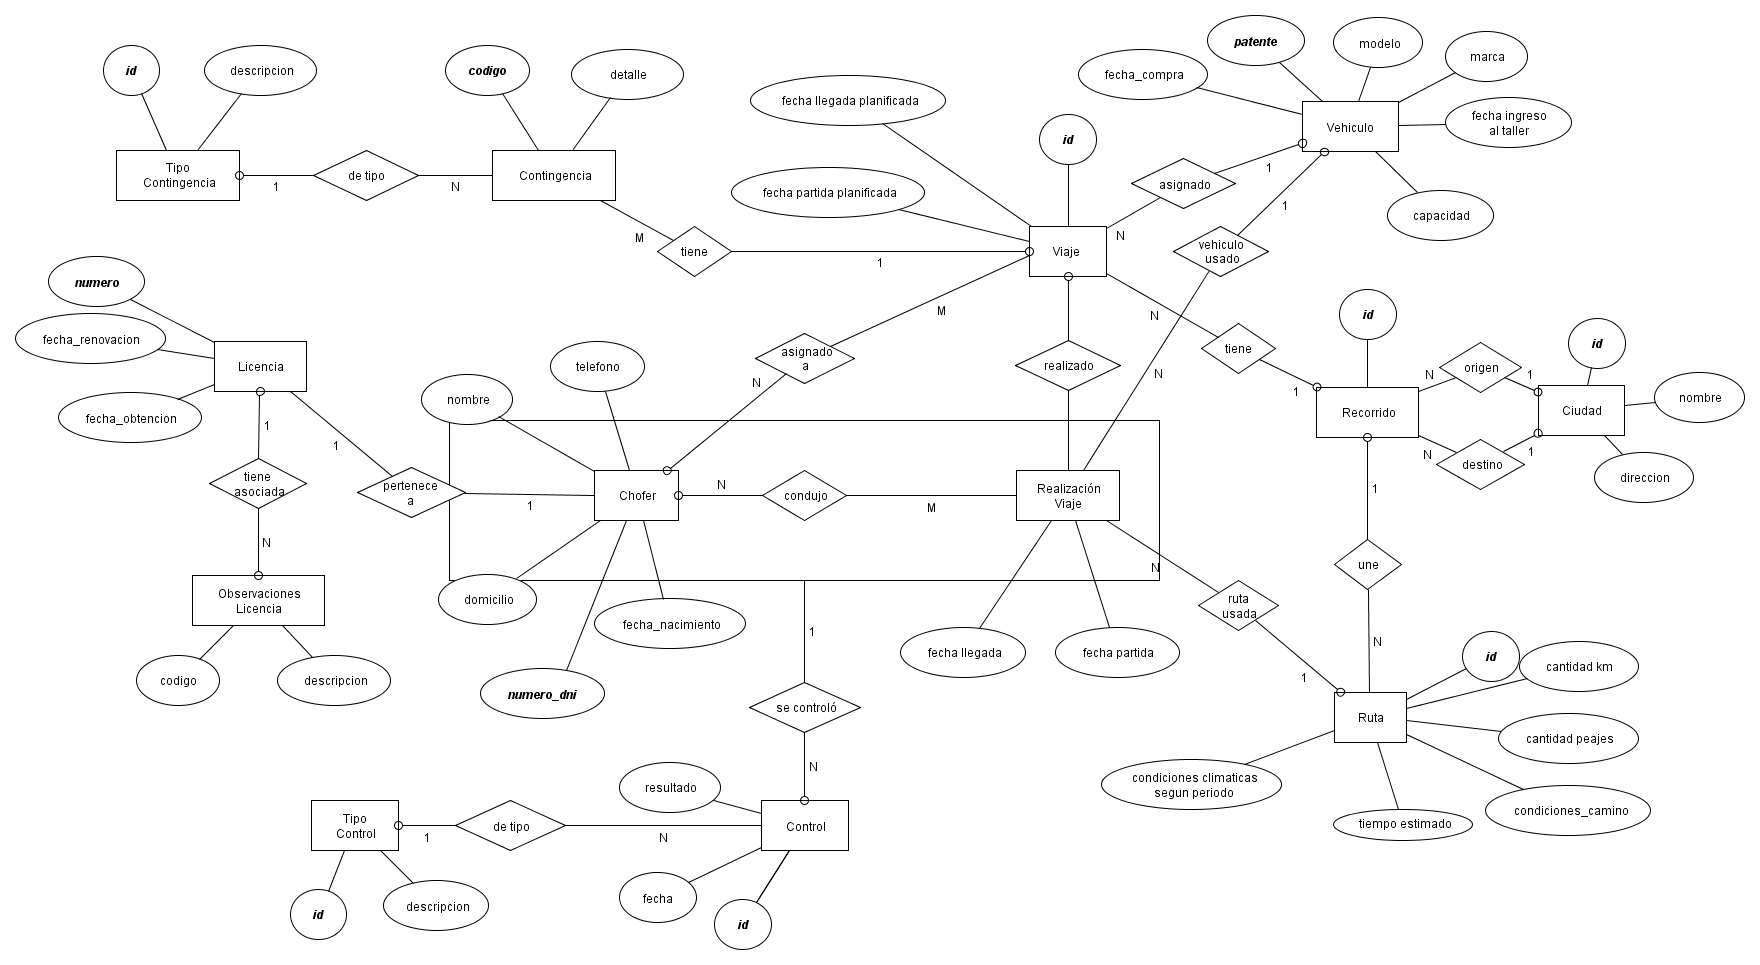
\includegraphics[angle=90,height=19.5cm]{../mer/mer.png}
			\label{fig:der}
		\end{figure}
\newpage


\subsection{Decisiones tomadas}
\begin{enumerate}
	\item Modelamos las observaciones como una entidad separada, por que en el dominio podr�a ser importante encontrar todos los choferes que usen anteojos, por ejemplo. Las observaciones se discriminan por estar tipificadas.
	\item La antig�edad del veh�culo, se deriva a partir de su fecha de compra.
	\item Se modela que no hay peajes poniendo un 0 y no consideramos que sea una entidad separada, pues no hay otra informaci�n relevante sobre ellos.
	\item En un principio hab�amos modelado el campo condiciones clim�ticas pens�ndolo como una relaci�n con un atributo asociado seg�n el periodo del a�o/condici�n clim�tica, sin embargo descartamos esta soluci�n pues nos hacia modelar cosas por dem�s que no encontramos necesario seg�n en el enunciado.
	\item Modelamos los viajes realizados asoci�ndolos a un viaje, para no perder la informaci�n de un viaje planificado al realizarlo y mantener la relaci�n entre estos.
	\item Como constraint la aridad de la relaci�n chofer asignado a viaje planificado es como m�ximo tres choferes asignados a un viaje planificado.
	\item En los veh�culos, asumimos que el estado es si est� en reparaci�n o no, y no algo adicional. Un veh�culo se encuentra en reparaci�n si tiene fecha de ingreso al taller. No guardamos el historial de reparaciones realizadas. 
	\item En nuestro modelo los viajes realizados puede haber sido hechos por choferes con licencias vencidas. Si model�ramos esto nos limitar�a muchas situaciones posibles validas. Adem�s como no guardamos historial de licencias, no podemos saber si hizo un viaje con la licencia vencida.
	\item La planificaci�n de los viajes se realiza en funci�n de un solo veh�culo. 
	\item Tanto el veh�culo como el chofer de un viaje realizado pueden ser diferentes a los propuestos durante la planificaci�n.
	\item Para guardar la informaci\'on sobre los viajes planificados una vez que ser realizan, los modelamos como tablas distintas. La PK del viaje realizado es la FK al viaje planificado.
\end{enumerate}

\section{MR}

\subsection{Esquema}

\textbf{TipoContingencia}(\underline{id}, descripci\'on)

PK = CK = \{idTipoContingencia\}
\medskip


\textbf{Contingencia}(\underline{c\'odigo}, descripci\'on, \dashuline{idTipoContingencia}, \dashuline{idViaje})

PK = CK =\{c\'odigo\}

FK = \{idTipoContingencia, idViaje\}
\medskip 

\textbf{Viaje}(\underline{idViaje}, fechaPartidaPlanificada, fechaLlegadaPlanificada ,\dashuline{idRecorrido}, \dashuline{idVehiculo} )

PK = CK = \{idViaje\}

FK = \{ idRecorrido, idVehiculo\}
\medskip 


\textbf{RealizacionViaje}(\underline{\dashuline{idViaje}}, fechaPartida, fechaLlegada ,\dashuline{idRuta}, \dashuline{idVehiculo} )

PK = CK = \{idViaje\}

FK = \{ idViaje, idRuta, idVehiculo\}
\medskip 

\textbf{Vehiculo}(\underline{patente}, fechaDeCompra, modelo, marca, capacidad, fechaDeIngresoAlTaller)

PK = CK =\{patente\}

FK = \{\}
\medskip 

\textbf{Recorrido}(\underline{idRecorrido},\dashuline{idCiudadOrigen}, \dashuline{idCiudadDestino} )

PK = CK =\{idRecorrido\}

FK = \{idCiudadOrigen, idCuidadDestino\}
\medskip

\textbf{Ciudad}(\underline{idCiudad}, nombre, direcci\'on )

PK = \{idCiudad\}

CK =\{direccion\}

FK = \{\}
\medskip


\textbf{Ruta}(\underline{idRuta}, cantidadKm, cantidadPeajes, condicionesCamino, tiempoEstimado, condicionesClimaticasSegunPeriodo )

PK = CK =\{idRuta\}

FK = \{\}
\medskip


\textbf{Control}(\underline{idControl}, resultado, fecha,\dashuline{idTipoControl}, \dashuline{idChofer}, \dashuline{idViaje}  )

PK = CK =\{idControl\}

FK = \{(idChofer,idViaje), idTipoControl\}
\medskip

\textbf{TipoControl}(\underline{idTipoControl}, descripcion  )

PK = CK =\{idTipoControl\}

FK = \{\}
\medskip

\textbf{Licencia}(\underline{numero}, fechaRenovacion, fechaObtencion  )

PK = CK =\{numero\}

FK = \{\}
\medskip


\textbf{ObservacionLicencia}(\underline{codigo}, descripcion,  )

PK = CK =\{codigo\}

FK = \{\}
\medskip

\textbf{TieneAsociada}(\underline{idLicencia}, \underline{idObservacionLicencia}  )

PK = CK =\{(idLicencia, idObservacionLicencia)\}

FK = \{idLicencia, idObservacionLicencia\}
\medskip

\textbf{Chofer}(\underline{codigo}, descripcion, \dashuline{idLiciencia} )

PK = CK =\{codigo\}

FK = \{idLiciencia\}
\medskip

\textbf{AsignadoA}(\underline{idChofer}, \underline{idViaje}  )

PK = CK =\{(idLicencia, idObservacionLicencia)\}

FK = \{idLicencia, idObservacionLicencia\}
\medskip

\textbf{Conduce}(\underline{idChofer}, \underline{idViajeRealizado}  )

PK = CK =\{(idChofer, idViajeRealizado)\}

FK = \{idChofer, idViajeRealizado\}
\medskip









\section{SQL}

\subsection{Stored Procedures}
		\lstinputlisting{../sql/procedures.sql}

		\bigskip
		\bigskip
\subsection{Triggers}
		\lstinputlisting{../sql/triggers.sql}
		
		\newpage
\subsection{Dise�o F�sico}
		\begin{figure}[ht!]
			\noindent\hspace*{-1cm}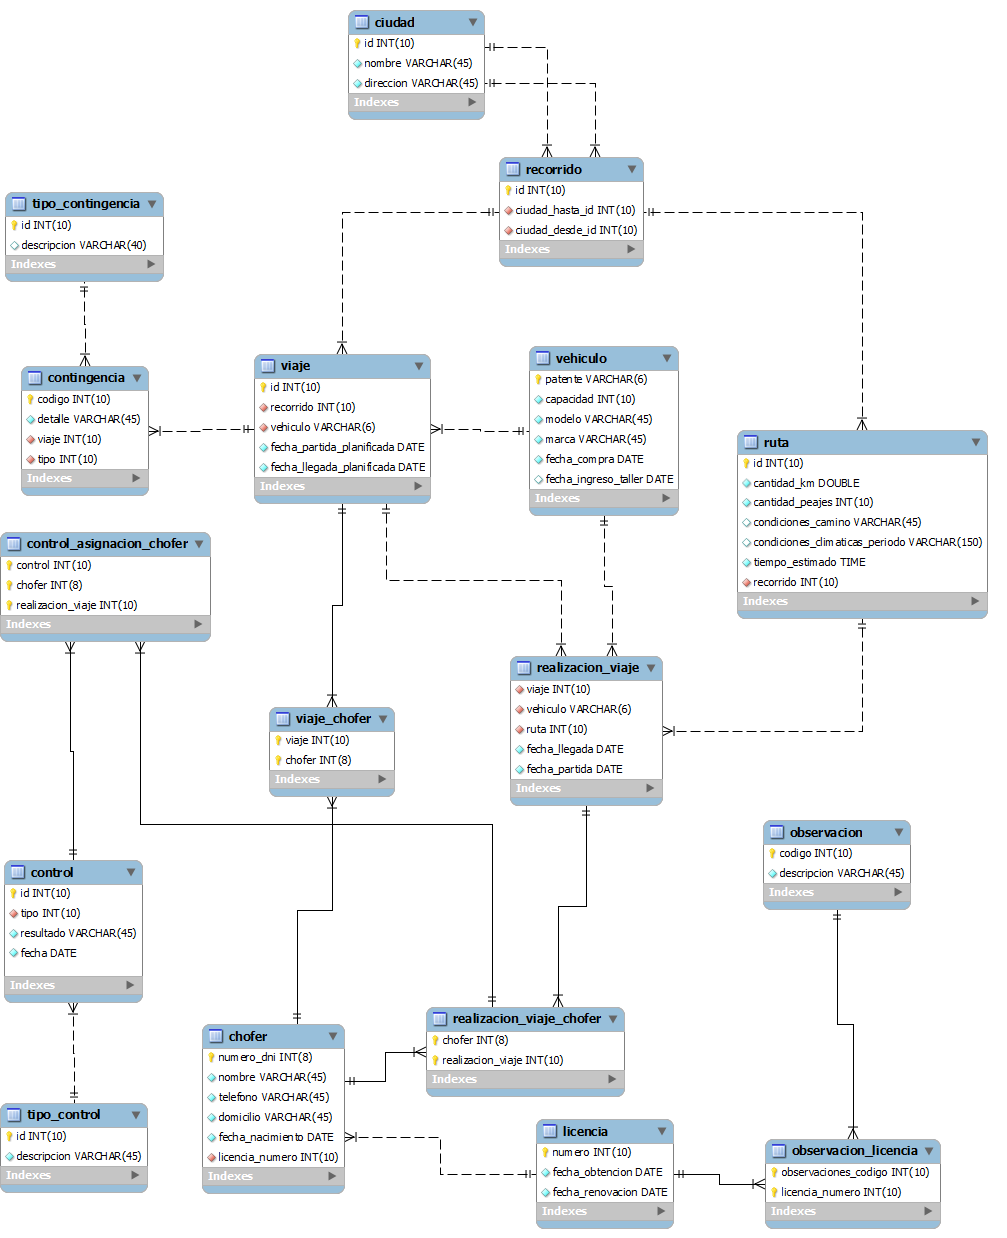
\includegraphics[height=20cm]{../model.png}
			\label{fig:fisico}
		\end{figure}
		
		\lstinputlisting{../sql/structure.sql}

\end{document}